\section{interpolators}
\paragraph{functions are:}
\begin{itemize}
  \item{lerp(linear interpolation): which works with 1D , 2D, 3D coordinates.}
  \item{clamp: ensure a value lies in a certian range. only 1D when writing this.}
  \item{smoothstep function.}
\end{itemize}

\paragraph{gfx::lerp}
  Our 1D version gfx::lerp accepts (start denoted by a, end denoted by b, progress denoted by t, between [0, 1]) and is implemeted like that
  $$lerp(a, b, t) = a + (b - a) * t$$
  gfx::lerp in other dimentions does the same for each axis.

\paragraph{gfx::clamp}
  gfx::clamp accepts (value v, minimum, maximum) and return max if v greater then max, and min when v smaller than min.
  and v if it lies in between min and max.

\paragraph{gfx::smoothstep}
  This is just an ease function that gives lerp smooth motion when applied to lerp t parameter.\\
  let smoothstep function be st for short.
  \Large{$$st(t) = 3t^{2} - 2t^{3}$$}

Our smoothstep function looks like this:-  \\\\\\\\
  \begin{center}
    \begin{tikzpicture}[transform canvas={scale=2.25}]
      \draw (-0.5, 0) -- (-0.5, 1) node[above, scale=0.4 ]{$y$};
      \draw (-0.5, 0) -- (0.5, 0)  node[above, scale=0.4 ]{$x$};
      \draw (-0.5, 0) -- (-0.45, 0.00725) -- (-0.4, 0.028) -- (-0.35, 0.06075) -- (-0.3, 0.104) -- (-0.25, 0.15625) -- (-0.2, 0.216) -- (-0.15, 0.28175) -- (-0.1, 0.352) -- (-0.05, 0.42525) -- (5.96046e-08, 0.5) -- (0.0500001, 0.57475) -- (0.1, 0.648) -- (0.15, 0.71825) -- (0.2, 0.784) -- (0.25, 0.84375) -- (0.3, 0.896) -- (0.35, 0.93925) -- (0.4, 0.972) -- (0.45, 0.99275);
    \end{tikzpicture}
  \end{center}

I think it looks nice. you may have noticed that this functions controls speed and by looking to the last figure
you can notice that the speed ease in and ease out which results in a motion that looks like something is sliding. \\

\subsection{gfx::cubic namespace}
This is a very small namespace to use cubic ease functions in, out and inout (prefixed with ease\_ ex: ease\_in). \\
gfx::cubic::ease\_in 
\Large{$$f(x) = x^{3}$$}  \\\\\\

  \begin{center}
    \begin{tikzpicture}[transform canvas={scale=2.25}]
      \draw (-0.5, 0) -- (-0.5, 1) node[above, scale=0.4 ]{$y$};
      \draw (-0.5, 0) -- (0.5, 0)  node[above, scale=0.4 ]{$x$};
      \draw (-0.5, 0) -- (-0.45, 0.000125) -- (-0.4, 0.001) -- (-0.35, 0.003375) -- (-0.3, 0.008) -- (-0.25, 0.015625) -- (-0.2, 0.027) -- (-0.15, 0.042875) -- (-0.1, 0.064) -- (-0.05, 0.091125) -- (5.96046e-08, 0.125) -- (0.0500001, 0.166375) -- (0.1, 0.216) -- (0.15, 0.274625) -- (0.2, 0.343) -- (0.25, 0.421875) -- (0.3, 0.512) -- (0.35, 0.614125) -- (0.4, 0.729) -- (0.45, 0.857375);

    \end{tikzpicture}
  \end{center}

gfx::cubic::ease\_out 
\Large{$$f(x) = 1 - (1 - x)^{3}$$} \\\\\\

  \begin{center}
    \begin{tikzpicture}[transform canvas={scale=2.25}]
      \draw (-0.5, 0) -- (-0.5, 1) node[above, scale=0.4 ]{$y$};
      \draw (-0.5, 0) -- (0.5, 0)  node[above, scale=0.4 ]{$x$};
      \draw (-0.5, 0) -- (-0.45, 0.142625) -- (-0.4, 0.271) -- (-0.35, 0.385875) -- (-0.3, 0.488) -- (-0.25, 0.578125) -- (-0.2, 0.657) -- (-0.15, 0.725375) -- (-0.1, 0.784) -- (-0.05, 0.833625) -- (5.96046e-08, 0.875) -- (0.0500001, 0.908875) -- (0.1, 0.936) -- (0.15, 0.957125) -- (0.2, 0.973) -- (0.25, 0.984375) -- (0.3, 0.992) -- (0.35, 0.996625) -- (0.4, 0.999) -- (0.45, 0.999875);
    \end{tikzpicture}
  \end{center}

gfx::cubic::ease\_inout \\
when x $<$ 0.5:
$$f(x) = 4x^3$$
when x $\geq$ 0.5:
$$f(x) = 1 - \frac{(2 - 2x)^3}{2}$$ \\\\\\
  \begin{center}
    \begin{tikzpicture}[transform canvas={scale=2.25}]
      \draw (-0.5, 0) -- (-0.5, 1) node[above, scale=0.4 ]{$y$};
      \draw (-0.5, 0) -- (0.5, 0)  node[above, scale=0.4 ]{$x$};
      \draw (-0.5, 0) -- (-0.45, 0.0005) -- (-0.4, 0.004) -- (-0.35, 0.0135) -- (-0.3, 0.032) -- (-0.25, 0.0625) -- (-0.2, 0.108) -- (-0.15, 0.1715) -- (-0.1, 0.256) -- (-0.05, 0.3645) -- (5.96046e-08, 0.5) -- (0.0500001, 0.6355) -- (0.1, 0.744) -- (0.15, 0.8285) -- (0.2, 0.892) -- (0.25, 0.9375) -- (0.3, 0.968) -- (0.35, 0.9865) -- (0.4, 0.996) -- (0.45, 0.9995);
    \end{tikzpicture}
  \end{center}

actually this is just a steeper version of our smoothstep function
